\documentclass[10pt]{article}
\usepackage[ngerman]{babel}
\usepackage[utf8]{inputenc}
\usepackage[T1]{fontenc}
\usepackage{amsmath}
\usepackage{amsfonts}
\usepackage{amssymb}
\usepackage[version=4]{mhchem}
\usepackage{stmaryrd}
\usepackage{graphicx}
\usepackage[export]{adjustbox}
\graphicspath{ {./images/} }

\begin{document}
\section*{Lineare Regression}
\section*{Definition}
Gegeben sind Datenpunkte $\left(x_{i} ; y_{i}\right)$ mit $1 \leq i \leq n$. Die Residuen oder Fehler $\epsilon_{i}=y_{i}-\underbrace{g\left(x_{i}\right)}_{=\hat{y}_{i}}$ dieser Datenpunkte sind die Abstände in $y$ Richtung zwischen den beobachteten Werten $y_{i}$ und den durch die lineare Regression prognostizierten Werten $\hat{y}_{i}=g\left(x_{i}\right)$. Die Ausgleichsoder Regressionsgerade $g(x)=m \cdot x+d$ (in $y$-Richtung) ist diejenige Gerade, für die die Summe der quadrierten Residuen $\sum_{i=1}^{n} \epsilon_{i}{ }^{2}$ am kleinsten ist.\\
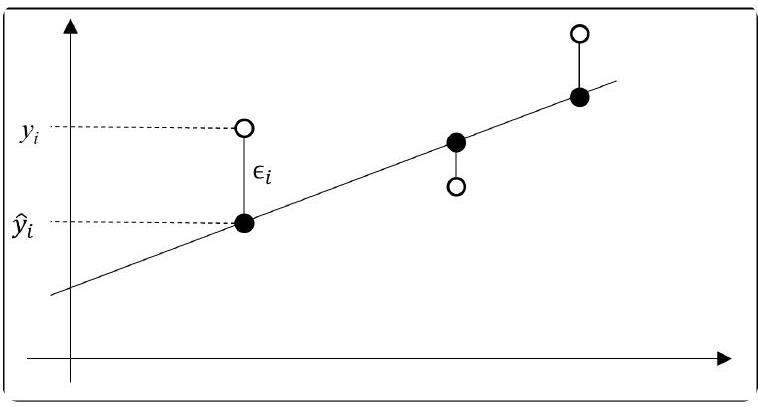
\includegraphics[width=\linewidth]{images/2025_01_02_5da43d4a2289c00b2d0dg-1}

\begin{verbatim}
Zusammenfassung Regressionsgerade:
Die Regressionsgerade $g(x)=m \cdot x+d$ mit den Parametern $m$ und $d$ ist die Gerade,
für die die Residualvarianz $\tilde{s}_{\epsilon}^{2}$ minimal ist.
Die Regressionsgerade hat die Steigung $m=\frac{\tilde{s}_{x y}}{\tilde{s}_{x}^{2}}$
und den $y$-Achsenabschnitt $d=\bar{y}-m \cdot \bar{x}$
Für die zugehörige (minimale) Residualvarianz gilt: $\tilde{s}_{\epsilon}^{2}=\tilde{s}_{y}^{2}-\frac{\tilde{s}_{x y}^{2}}{\tilde{s}_{x}^{2}}$
mit:
Varianz der $x_{i}$-Werte: $\tilde{s}_{x}^{2}$
Varianz. der $y_{i}$-Werte (Totale Varianz) : $\tilde{s}_{y}^{2}$
Varianz der $\hat{y}_{i}$-Werte (Prognostizierte Varianz): $\tilde{s}_{\hat{y}}^{2}$
Kovarianz: $\tilde{s}_{x y}$
arithmetische Mittelwerte $\bar{x}$ und $\bar{y}$
Hinweis: Die Berechnungen können alternativ auch mit den korrigierten Varianzen $s_{\epsilon}^{2}$,
$s_{x}^{2}, s_{y}^{2}, s_{\hat{y}}^{2}$ und der korrigierten Kovarianz $s_{x y}$ erfolgen!
\end{verbatim}

\section*{Zusammenfassung Bestimmtheitsmass:}
Die Totale Varianz setzt sich zusammen aus der Residualvarianz und der Varianz der prognostizierten Werte (Varianzzerlegung):

$$
\tilde{s}_{y}^{2}=\tilde{s}_{\epsilon}^{2}+\underbrace{\tilde{s}_{\hat{y}}^{2}} \frac{\tilde{s}_{x y}^{2}}{\tilde{s}_{x}^{2}}
$$

Das Bestimmtheitsmass $R^{2}$ beurteilt die globale Anpassungsgüte einer Regression über den Anteil der prognostizierten (erklärten) Varianz $\tilde{s}_{\hat{y}}^{2}$ an der totalen Varianz $\tilde{s}_{y}^{2}$ : $R^{2}=\frac{\tilde{s}_{\tilde{y}}^{2}}{\tilde{s}_{y}^{2}}$ bzw. $R^{2}=\frac{s_{y}^{2}}{s_{y}^{2}}$

Das Bestimmtheitsmass $R^{2}$ stimmt überein mit dem Quadrat des Korrelationskoeffizienten (nach Bravais-Pearson):\\
$R^{2}=\frac{\tilde{s}_{x y}^{2}}{\tilde{s}_{x}^{2} \cdot \tilde{s}_{y}^{2}}=r_{x y}^{2}$ bzw. $R^{2}=\frac{s_{x y}^{2}}{s_{x}^{2} \cdot s_{y}^{2}}=r_{x y}^{2}$

\section*{Bestimmung der Regressionsgerade als Matrizenproblem:}
Die Parameter $m$ und $d$ werden mit der Matrix $A=\left(\begin{array}{cc}x_{1} & 1 \\ x_{2} & 1 \\ \vdots & \vdots \\ x_{n} & 1\end{array}\right)$ aus den folgenden Normalengleichungen berechnet:

$$
A^{T} \cdot A \cdot\binom{m}{q}=A^{T} \cdot\left(\begin{array}{c}
y_{1} \\
\vdots \\
y_{n}
\end{array}\right)
$$

\section*{Die Methode der kleinsten Quadrate (KQM)}
Das lineare, inhomogene Gleichungssystem mit $m$ Gleichungen und $n$ Unbekannten $x_{1}, \ldots, x_{n}$

$$
\left.\begin{array}{ccccccc}
a_{11} x_{1} & +a_{12} x_{2} & +\ldots & +a_{1 n} x_{n} & = & y_{1}+\epsilon_{1} \\
a_{21} x_{1} & +a_{22} x_{2} & +\ldots & + & a_{2 n} x_{n} & = & y_{2}+\epsilon_{2} \\
\vdots & \vdots & & & \vdots & & \vdots \\
a_{m 1} x_{1} & +a_{m 2} x_{2} & +\ldots & +a_{m n} x_{n} & =y_{m}+\epsilon_{m}
\end{array}\right\} \Leftrightarrow \underbrace{\left(\begin{array}{cccc}
a_{11} & a_{12} & \ldots & a_{1 n} \\
a_{21} & a_{22} & \ldots & a_{2 n} \\
\vdots & \vdots & & \vdots \\
a_{m 1} & a_{m 2} & \ldots & a_{m n}
\end{array}\right)}_{=A} \cdot \underbrace{\left(\begin{array}{c}
x_{1} \\
x_{2} \\
\vdots \\
x_{n}
\end{array}\right)}_{=\vec{x}}=\underbrace{\left(\begin{array}{c}
y_{1} \\
y_{2} \\
\vdots \\
y_{m}
\end{array}\right)}_{=\vec{y}}+\underbrace{\left(\begin{array}{c}
\epsilon_{1} \\
\epsilon_{2} \\
\vdots \\
\epsilon_{m}
\end{array}\right)}_{=\vec{\epsilon}}
$$

hat immer (mind.) eine Lösung mit einem Residuenvektor $\vec{\epsilon}$ von minimalem Betrag. Diese Lösungen sind Lösungen der\\
Normalengleichungen $A^{T} \cdot A \cdot \vec{x}=A^{T} \cdot \vec{y}$.\\
Hat die Matrix $A$ den Rang $n$, so ist die symmetrische $n \times n$ Matrix $A^{T} \cdot A$ invertierbar und die einzige Lösung erhält man aus der Gleichung $\vec{x}=\left(A^{T} \cdot A\right)^{-1} \cdot A^{T} \vec{y}$.

Für die Lösungen $\vec{x}$ gilt immer:

\begin{itemize}
  \item $\quad A \cdot \vec{x}$ und der Residuenvektor $\vec{\epsilon}=\vec{y}-A \cdot \vec{x}$ sind orthogonal zueinander.
  \item Es gilt der Satz von Pythagoras (Quadratsummenzerlegung):
\end{itemize}

$$
|\vec{y}|^{2}=|A \cdot \vec{x}|^{2}+\underbrace{|\vec{y}-A \cdot \vec{x}|^{2}}_{=|\vec{\epsilon}|^{2}}
$$

Zuletzt geändert: Montag, 11. Dezember 2023, 15:51\\
4. Zusammenfassung: Spezielle Verteilungen

Direkt zu:\\
7. und 8. Zusammenfassung: Schliessende Statistik

\section*{Datenschutz | $\square$ Supportanfrage}

\end{document}